\documentclass[11pt,a4paper]{article}
\usepackage[utf8]{inputenc}
\usepackage[vietnamese]{babel}
\usepackage{amsmath,amssymb}
\usepackage[version=4]{mhchem}
\usepackage{geometry}
\geometry{top=0.9cm,bottom=0.9cm,left=1.35cm,right=1.35cm,headheight=24pt,headsep=5pt,footskip=11pt}
\usepackage{graphicx}
\usepackage{xcolor}
\usepackage{tabularx}
\usepackage{array}
\usepackage{tikz}
\usepackage{multicol}
\usepackage{fancyhdr}
\usepackage{enumitem}

\definecolor{hfRed}{HTML}{D32F2F}
\definecolor{hfGreen}{HTML}{8BC390}
\definecolor{mainGreen}{HTML}{2E7D32}

\usepackage{ex_test}

\pagestyle{fancy}
\fancyhf{}
\renewcommand{\headrulewidth}{0.75pt}
\renewcommand{\headrule}{\hbox to\headwidth{\color{hfGreen}\leaders\hrule height \headrulewidth\hfill}}
\renewcommand{\footrulewidth}{0.75pt}
\renewcommand{\footrule}{\hbox to\headwidth{\color{hfGreen}\leaders\hrule height \footrulewidth\hfill}}

\fancyhead[L]{\small\itshape\color{hfRed}Tài liệu lưu hành nội bộ}
\fancyhead[R]{\small\color{hfRed}Thầy \textbf{TRẦN VĂN THẠNH} - 0777.470.803}

\fancyfoot[L]{\footnotesize\itshape\color{hfRed}CS1: 6/15 Nguyễn Hoàng, P. Kim Long, TP Huế \quad|\quad CS2: 24 Đặng Thái Thân, TP Huế}
\fancyfoot[R]{\small\textbf{\color{hfRed}Trang \thepage}}

\setlength{\parindent}{0pt}
\setlength{\parskip}{0.0pt}

\def\loigiai#1{}

\begin{document}

\Opensolutionfile{ans}[ans-de13-hs]

\noindent
\begin{minipage}[t]{0.48\textwidth}
	\textbf{SỞ GIÁO DỤC VÀ ĐÀO TẠO THỪA THIÊN HUẾ}\\
	\textbf{TRƯỜNG THPT HAI BÀ TRƯNG}\\
	\textbf{ĐỀ CHÍNH THỨC}\\
	\textit{(Đề thi có 04 trang)}
\end{minipage}\hfill
\begin{minipage}[t]{0.48\textwidth}
	\raggedleft
	\textbf{\color{mainGreen}ĐỀ KIỂM TRA ĐỊNH KỲ CHƯƠNG 5 (PIN ĐIỆN – ĐIỆN PHÂN)}\\
	\textbf{MÔN: HOÁ HỌC -- LỚP 12}\\
	\textit{Thời gian làm bài: 50 phút (không kể thời gian phát đề)}\\
	\textbf{Mã đề thi: 113}
\end{minipage}


\vspace{1pt}
\noindent\textit{Họ, tên thí sinh: \dots\dots\dots\dots\dots\dots\dots\dots\dots\dots\dots\dots\dots\dots\dots\dots\dots\dots\dots\dots\dots\dots Lớp: \dots\dots\dots\dots SBD: \dots\dots\dots\dots}\\
\noindent\textit{(Cho biết nguyên tử khối: H = 1; C = 12; N = 14; O = 16; Na = 23; Mg = 24; Al = 27; S = 32; Cl = 35,5; K = 39; Ca = 40; Fe = 56; Ni = 59; Cu = 64; Zn = 65; Ag = 108; Sn = 119; Pb = 207; hằng số Faraday F = 96500 C/mol).}

\vspace{2pt}
\noindent
\textbf{PHẦN I (4,5 điểm -- 18 câu): Câu trắc nghiệm nhiều phương án lựa chọn.}\\
\textit{Thí sinh trả lời từ câu 1 đến câu 18. Mỗi câu hỏi thí sinh chỉ chọn một phương án.}

\setcounter{ex}{0}

\begin{ex}
(SBT -- CĐ). Sức điện động chuẩn của pin Galvani được tính như thế nào?
\choice
{Bằng hiệu của thế điện cực chuẩn tương ứng của điện cực dương và điện cực âm}
{Bằng tổng của thế điện cực chuẩn tương ứng của điện cực dương và điện cực âm}
{Bằng tích của thế điện cực chuẩn tương ứng của điện cực dương và điện cực âm}
{Bằng thương của thế điện cực chuẩn tương ứng của điện cực dương và điện cực âm}
\loigiai{}
\end{ex}

\begin{ex}
(SBT -- KNTT). Trong pin điện hoá Zn -- Cu, phản ứng hoá học xảy ra giữa hai dạng nào của các cặp oxi hoá -- khử tương ứng?
\choice
{Zn và \ce{Cu^2+}}
{Zn và Cu}
{\ce{Zn^2+} và \ce{Cu^2+}}
{Pb và \ce{Cu^2+}}
\loigiai{}
\end{ex}

\begin{ex}
(SBT -- KNTT). Trong quá trình hoạt động của pin điện Zn -- Cu, dòng electron di chuyển từ
\choice
{cực kẽm sang cực đồng}
{cực bên phải sang cực bên trái}
{cathode sang anode}
{cực dương sang cực âm}
\loigiai{}
\end{ex}

\begin{ex}
(SBT -- KNTT). Phản ứng hoá học chính xảy ra trong quá trình điện phân nóng chảy \ce{Al2O3} trong cryolite (\ce{3NaF.AlF3}) là
\choice
{\ce{2AlF3 -> 2Al + 3F2}}
{\ce{2NaF -> 2Na + F2}}
{\ce{2H2O -> 2H2 + O2}}
{\ce{2Al2O3 -> 4Al + 3O2}}
\loigiai{}
\end{ex}

\begin{ex}
(SBT -- KNTT). Việc duy trì điện áp thấp ($\sim 5\text{ V}$) trong quá trình điện phân nóng chảy \ce{Al2O3} trong cryolite (\ce{3NaF.AlF3}) nhằm ngăn cản quá trình nào sau đây xảy ra ở cathode?
\choice
{\ce{Al^3+ + 3e -> Al}}
{\ce{Na+ + 1e -> Na}}
{\ce{F2 + 2e -> 2F-}}
{\ce{O2 + 4e -> 2O^2-}}
\loigiai{}
\end{ex}

\begin{ex}
(SBT -- KNTT). Trong công nghiệp, phương pháp điện phân dung dịch được sử dụng để sản xuất một lượng đáng kể kim loại nào sau đây?
\choice
{Zn}
{Al}
{Fe}
{Mg}
\loigiai{}
\end{ex}

\begin{ex}
(SBT -- CTST). Dãy kim loại sắp xếp theo chiều tăng dần tính khử từ trái sang phải là
\choice
{Pb, Ni, Sn, Zn}
{Pb, Sn, Ni, Zn}
{Ni, Sn, Zn, Pb}
{Ni, Zn, Pb, Sn}
\loigiai{}
\end{ex}

\begin{ex}
(SBT -- CTST). Dãy cation kim loại được sắp xếp theo chiều tăng dần tính oxi hóa từ trái sang phải là
\choice
{\ce{Cu^2+}, \ce{Fe^2+}, \ce{Mg^2+}}
{\ce{Mg^2+}, \ce{Fe^2+}, \ce{Cu^2+}}
{\ce{Mg^2+}, \ce{Cu^2+}, \ce{Fe^2+}}
{\ce{Cu^2+}, \ce{Mg^2+}, \ce{Fe^2+}}
\loigiai{}
\end{ex}

\begin{ex}
(SBT -- KNTT). Phản ứng hoá học xảy ra trong pin điện hoá Sn -- Cu: $\ce{Sn + Cu^2+ -> Sn^2+ + Cu}$. Trong quá trình hoạt động của pin điện hoá, nhận định nào sau đây là đúng?
\choice
{Khối lượng của điện cực Sn tăng}
{Nồng độ \ce{Sn^2+} trong dung dịch tăng}
{Khối lượng của điện cực Cu giảm}
{Nồng độ \ce{Cu^2+} trong dung dịch tăng}
\loigiai{}
\end{ex}

\begin{ex}
(SBT -- KNTT). Một pin điện hoá có điện cực Zn nhúng trong dung dịch \ce{ZnSO4} và điện cực Cu nhúng trong dung dịch \ce{CuSO4}. Sau một thời gian pin đó phóng điện thì
\choice
{khối lượng điện cực Zn giảm còn khối lượng điện cực Cu tăng}
{khối lượng điện cực Zn tăng còn khối lượng điện cực Cu giảm}
{khối lượng cả hai điện cực Zn và Cu đều tăng}
{khối lượng cả hai điện cực Zn và Cu đều giảm}
\loigiai{}
\end{ex}

\newpage

\begin{ex}
(SBT -- KNTT). Khi điện phân dung dịch gồm \ce{CuSO4} và \ce{HCl} (sử dụng điện cực trơ, có màng ngăn xốp), chất khí đầu tiên thoát ra ở anode là
\choice
{\ce{O2}}
{\ce{Cl2}}
{\ce{H2}}
{\ce{SO2}}
\loigiai{}
\end{ex}

\begin{ex}
(SBT -- CTST). Cách nào sau đây \textbf{không} được dùng để điều chế \ce{NaOH}?
\choice
{Điện phân dung dịch \ce{NaCl} có màng ngăn xốp, điện cực trơ}
{Cho dung dịch \ce{Ca(OH)2} tác dụng với dung dịch \ce{Na2CO3}}
{Cho \ce{Na2O} tác dụng với nước}
{Dẫn khí \ce{NH3} vào dung dịch \ce{Na2CO3}}
\loigiai{}
\end{ex}

\begin{ex}
(SBT -- CTST). Khi điện phân \ce{NaCl} nóng chảy (điện cực trơ), ở cathode xảy ra
\choice
{sự khử ion \ce{Cl-}}
{sự oxi hóa ion \ce{Cl-}}
{sự oxi hóa ion \ce{Na+}}
{sự khử ion \ce{Na+}}
\loigiai{}
\end{ex}

\begin{ex}
(SBT -- CTST). Khi điện phân \ce{CaCl2} nóng chảy (điện cực trơ), ở anode xảy ra
\choice
{sự khử ion \ce{Cl-}}
{sự khử ion \ce{Ca^2+}}
{sự oxi hóa ion \ce{Ca^2+}}
{sự oxi hóa ion \ce{Cl-}}
\loigiai{}
\end{ex}

\begin{ex}
Một học sinh thực hiện ba thí nghiệm liên quan đến ba kim loại X, Y, Z và dung dịch muối nitrate của chúng ở điều kiện chuẩn và quan sát được các hiện tượng sau:\\
(1) X không phản ứng được với dung dịch \ce{Y(NO3)2} 1 M.\\
(2) Y tan trong dung dịch muối \ce{ZNO3} 1 M và xuất hiện tinh thể Z.\\
(3) Z không phản ứng với dung dịch \ce{X(NO3)2} 1 M.\\
Trật tự nào sau đây thể hiện đúng mức độ khử của ba kim loại?
\choice
{$\text{X} > \text{Y} > \text{Z}$}
{$\text{Y} > \text{X} > \text{Z}$}
{$\text{X} > \text{Z} > \text{Y}$}
{$\text{Y} > \text{Z} > \text{X}$}
\loigiai{}
\end{ex}

\begin{ex}
(SBT -- CTST). Cho $E^\circ_{\text{Pin(Ni-Cu)}} = 0{,}59\text{ V}$ và $E^\circ_{\ce{Cu^2+/Cu}} = 0{,}34\text{ V}$. Thế điện cực chuẩn của cặp oxi hóa -- khử \ce{Ni^2+/Ni} ($E^\circ_{\ce{Ni^2+/Ni}}$) là
\choice
{0,34 V}
{0,35 V}
{-0,34 V}
{-0,25 V}
\loigiai{}
\end{ex}

\begin{ex}
(SBT -- KNTT). Sức điện động chuẩn của pin điện hoá \ce{H2} -- Cu (gồm hai điện cực ứng với hai cặp oxi hoá -- khử là \ce{2H+/H2} và \ce{Cu^2+/Cu}) đo được bằng vôn kế có điện trở vô cùng lớn là 0,340 V. Từ đó, xác định được thế điện cực chuẩn của cặp \ce{Cu^2+/Cu} là
\choice
{-0,340 V}
{0,000 V}
{0,680 V}
{+0,340 V}
\loigiai{}
\end{ex}

\begin{ex}
(SBT -- CTST). Điện phân một dung dịch hỗn hợp gồm: \ce{HCl}, \ce{CuCl2}, \ce{NaCl} với điện cực trơ, có màng ngăn. Kết luận nào sau đây \textbf{không} đúng?
\choice
{Sau khi kết thúc quá trình điện phân, pH của dung dịch tăng so với dung dịch ban đầu}
{Các chất bị điện phân lần lượt theo thứ tự: \ce{CuCl2}, \ce{HCl}, \ce{NaCl} và \ce{H2O}}
{Quá trình điện phân \ce{NaCl} làm tăng pH của dung dịch}
{Quá trình điện phân \ce{HCl} làm giảm pH của dung dịch}
\loigiai{}
\end{ex}

\newpage

\noindent
\textbf{PHẦN II (4,0 điểm -- 4 câu): Câu trắc nghiệm đúng sai.}\\
\textit{Thí sinh trả lời từ câu 1 đến câu 4. Trong mỗi ý a), b), c), d) ở mỗi câu, thí sinh chọn đúng hoặc sai.}

\setcounter{ex}{0}

\begin{ex}
Cho thế điện cực chuẩn của các cặp oxi hóa – khử: $E^\circ_{\ce{Cu^2+/Cu}} = 0{,}34\text{ V}$; $E^\circ_{\ce{Fe^2+/Fe}} = -0{,}44\text{ V}$; $E^\circ_{\ce{Fe^3+/Fe^2+}} = 0{,}77\text{ V}$; $E^\circ_{\ce{Ag+/Ag}} = 0{,}80\text{ V}$. Các phản ứng có thể xảy ra là:
\choiceTF
{\ce{Cu^2+ + Fe -> Cu + Fe^2+}}
{\ce{Fe + 2Fe^3+ -> 3Fe^2+}}
{\ce{Ag+ + Fe^2+ -> Ag + Fe^3+}}
{\ce{Cu + 2Fe^3+ -> Cu^2+ + 2Fe^2+}}
\loigiai{}
\end{ex}

\begin{ex}
(SBT – KNTT). Xét quá trình hoạt động của một pin điện hoá Cu – Ag được thiết lập ở các điều kiện như hình vẽ bên. Cho thế điện cực chuẩn của các cặp \ce{Cu^2+/Cu} và \ce{Ag+/Ag} lần lượt là $+0{,}340\text{ V}$ và $+0{,}799\text{ V}$.
\par\vspace{2pt}{\centering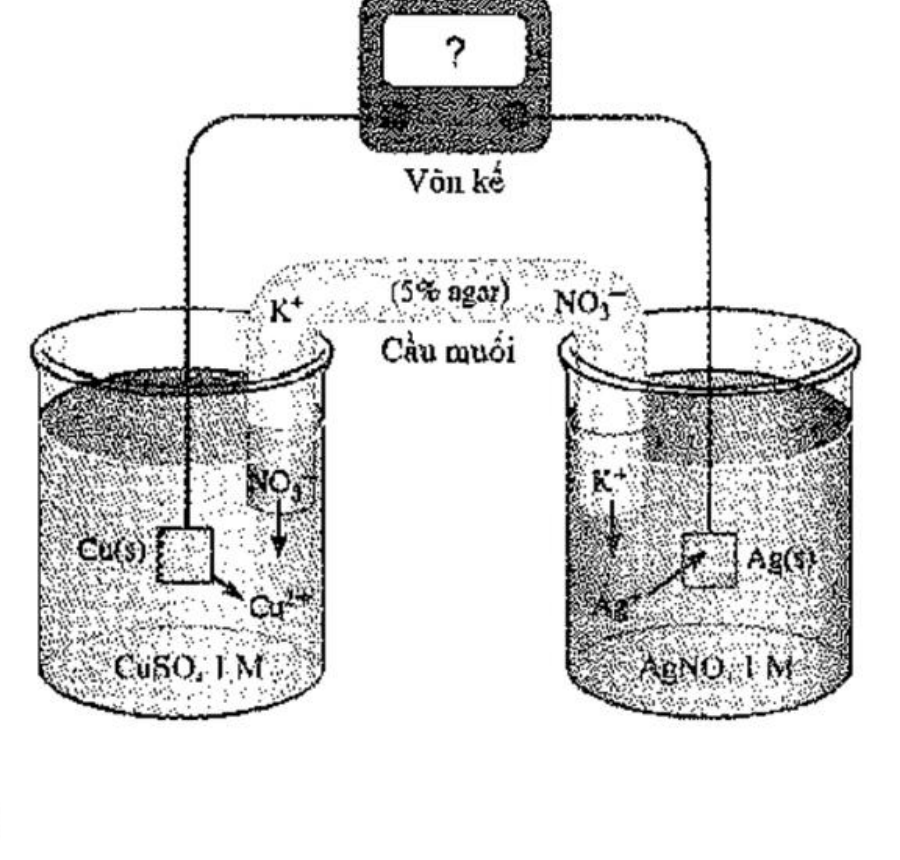
\includegraphics[height=2.3cm]{images_crop_de13/p2_cau2_pin_cu_ag.png}\par}\vspace{2pt}
\choiceTF
{Giá trị sức điện động chuẩn của pin điện hoá trên là 0,459 V}
{Ở anode xảy ra quá trình oxi hoá Cu, ở cathode xảy ra quá trình khử \ce{Ag+}}
{Điện cực Cu tăng khối lượng, điện cực Ag giảm khối lượng}
{Phản ứng hoá học xảy ra trong pin: \ce{Cu + 2Ag+ -> Cu^2+ + 2Ag}}
\loigiai{}
\end{ex}

\begin{ex}
Thí nghiệm điện phân được thực hiện như hình vẽ sau:
\par\vspace{2pt}{\centering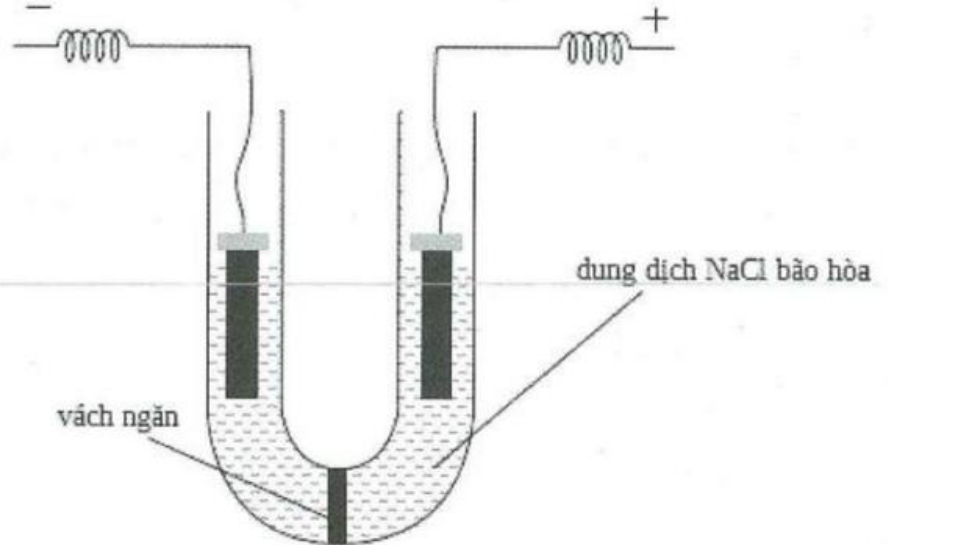
\includegraphics[height=2.1cm]{images_crop_de13/p2_cau3_dien_phan_nacl.png}\par}\vspace{2pt}
\choiceTF
{Có khí \ce{H2} thoát ra ở điện cực dương, khí \ce{O2} thoát ra ở cực âm}
{Thí nghiệm này ứng dụng để điều chế \ce{NaOH} trong công nghiệp}
{Nếu không có vách ngăn điện cực, dung dịch thu được có tính tẩy màu}
{Dung dịch sau điện phân làm quỳ tím chuyển sang màu xanh}
\loigiai{}
\end{ex}

\begin{ex}
Điện phân dung dịch \ce{MSO4} (M là kim loại) với điện cực trơ, cường độ dòng điện không đổi. Sau thời gian $t$ giây, thu được $a\text{ mol}$ khí ở anode. Nếu thời gian điện phân là $2t$ giây thì tổng số mol khí thu được ở cả hai điện cực là $2{,}5a\text{ mol}$. Giả sử hiệu suất điện phân là 100\%, khí sinh ra không tan trong nước.
\choiceTF
{Tại thời điểm $2t$ giây, có bọt khí ở cathode}
{Tại thời điểm $t$ giây, ion \ce{M^2+} chưa bị điện phân hết}
{Dung dịch sau điện phân có pH $< 7$}
{Khi thu được $1{,}8a\text{ mol}$ khí ở anode thì vẫn chưa xuất hiện bọt khí ở cathode}
\loigiai{}
\end{ex}

\newpage

\noindent
\textbf{PHẦN III (1,5 điểm -- 6 câu): Câu trắc nghiệm yêu cầu trả lời ngắn.}\\
\textit{Thí sinh trả lời từ câu 1 đến câu 6.}

\setcounter{ex}{0}

\begin{ex}
Có 3 cốc đựng các dung dịch muối có nồng độ 1 M, cho vào mỗi cốc 1 thanh Al:\\
(a) Cốc I: \ce{Pb(NO3)2} (aq)\quad (b) Cốc II: \ce{Ni(NO3)2} (aq)\quad (c) Cốc III: \ce{Cu(NO3)2} (aq)\\
Có bao nhiêu cốc có phản ứng xảy ra?
\par\noindent\textit{Trả lời:} \dotfill
\loigiai{}
\end{ex}

\begin{ex}
Cho pin điện hóa Zn -- Cu gồm hai cặp oxi hóa -- khử \ce{Zn^2+/Zn} và \ce{Cu^2+/Cu}. Cho thế điện cực chuẩn $E^\circ_{\ce{Cu^2+/Cu}} = 0{,}34\text{ V}$ và $E^\circ_{\ce{Zn^2+/Zn}} = -0{,}76\text{ V}$. Tính sức điện động chuẩn của pin (theo đơn vị V).
\par\noindent\textit{Trả lời:} \dotfill
\loigiai{}
\end{ex}

\begin{ex}
Điện phân dung dịch hỗn hợp gồm: \ce{NaCl}, \ce{Mg(NO3)2}, \ce{ZnCl2}, \ce{CuSO4} và \ce{Fe2(SO4)3} với điện cực trơ cho đến khi nước bắt đầu điện phân ở cả hai điện cực thì dừng lại. Thu được bao nhiêu chất rắn (kim loại) ở cathode?
\par\noindent\textit{Trả lời:} \dotfill
\loigiai{}
\end{ex}

\begin{ex}
Cho các phản ứng sau:\\
(1) Cho Cu vào dung dịch \ce{FeSO4}.\\
(2) Cho Cu vào dung dịch \ce{Fe2(SO4)3}.\\
(3) Cho K vào dung dịch \ce{CuSO4}.\\
(4) Cho dung dịch \ce{AgNO3} vào dung dịch \ce{Fe(NO3)2}.\\
Số lượng phản ứng có thể thu được đơn chất kim loại là
\par\noindent\textit{Trả lời:} \dotfill
\loigiai{}
\end{ex}

\begin{ex}
Cho một pin Galvani với điện cực Zn và Cu có sức điện động chuẩn là 1,10 V. Sử dụng pin này để thắp sáng một bóng đèn nhỏ với cường độ dòng điện chạy qua là $I = 0{,}02\text{ A}$. Nếu điện cực kẽm hao mòn 0,1 mol do pin phóng điện thì thời gian tối đa mà pin thắp sáng được bóng đèn là bao nhiêu giờ?\\
Cho biết công thức: $Q = n \cdot F = I \cdot t$, trong đó $Q$ là điện lượng (C), $n$ là số mol electron đi qua dây dẫn, $I$ là cường độ dòng điện (A), $t$ là thời gian (giây), $F$ là hằng số Faraday ($F = 96500\text{ C/mol}$). (Làm tròn kết quả đến hàng đơn vị).
\par\noindent\textit{Trả lời:} \dotfill
\loigiai{}
\end{ex}

\begin{ex}
Tiến hành điện phân dung dịch \ce{CuSO4} với anode bằng đồng (hiện tượng dương cực tan). Để hoà tan $100\text{ g}$ đồng ở anode trong 8 giờ thì cần cường độ dòng điện bằng bao nhiêu ampe? (Làm tròn kết quả đến chữ số hàng phần mười).
\par\noindent\textit{Trả lời:} \dotfill
\loigiai{}
\end{ex}


\Closesolutionfile{ans}

\end{document}
